

% This document was generated by the publish-function
% from GNU Octave 5.2.0



\documentclass[10pt]{article}
\usepackage{listings}
\usepackage{mathtools}
\usepackage{amssymb}
\usepackage{graphicx}
\usepackage{hyperref}
\usepackage{xcolor}
\usepackage{titlesec}
\usepackage[utf8]{inputenc}
\usepackage[T1]{fontenc}
\usepackage{lmodern}


\lstset{
language=Octave,
numbers=none,
frame=single,
tabsize=2,
showstringspaces=false,
breaklines=true}


\titleformat*{\section}{\Huge\bfseries}
\titleformat*{\subsection}{\large\bfseries}
\renewcommand{\contentsname}{\Large\bfseries Contents}
\setlength{\parindent}{0pt}

\begin{document}

{\Huge\section*{pub\_example}}

\tableofcontents
\vspace*{4em}



\phantomsection
\addcontentsline{toc}{section}{Headline title}
\subsection*{Headline title}

\begin{lstlisting}
#
# Some *bold*, _italic_, or |monospaced| Text with
# a <https://www.octave.org link to *GNU Octave*>. ##
         # "Real" Octave commands to be evaluated
         sombrero ()
         # persistent ignored
#         eval('persistent calls1 = 0;')
#        if(calls1==0)
#         publish('/Users/zhanghongliang/Documents/Octave/FunctionsandScripts/pub_example.m')
#         calls1++
#         endif
\end{lstlisting}
\begin{figure}[!ht]
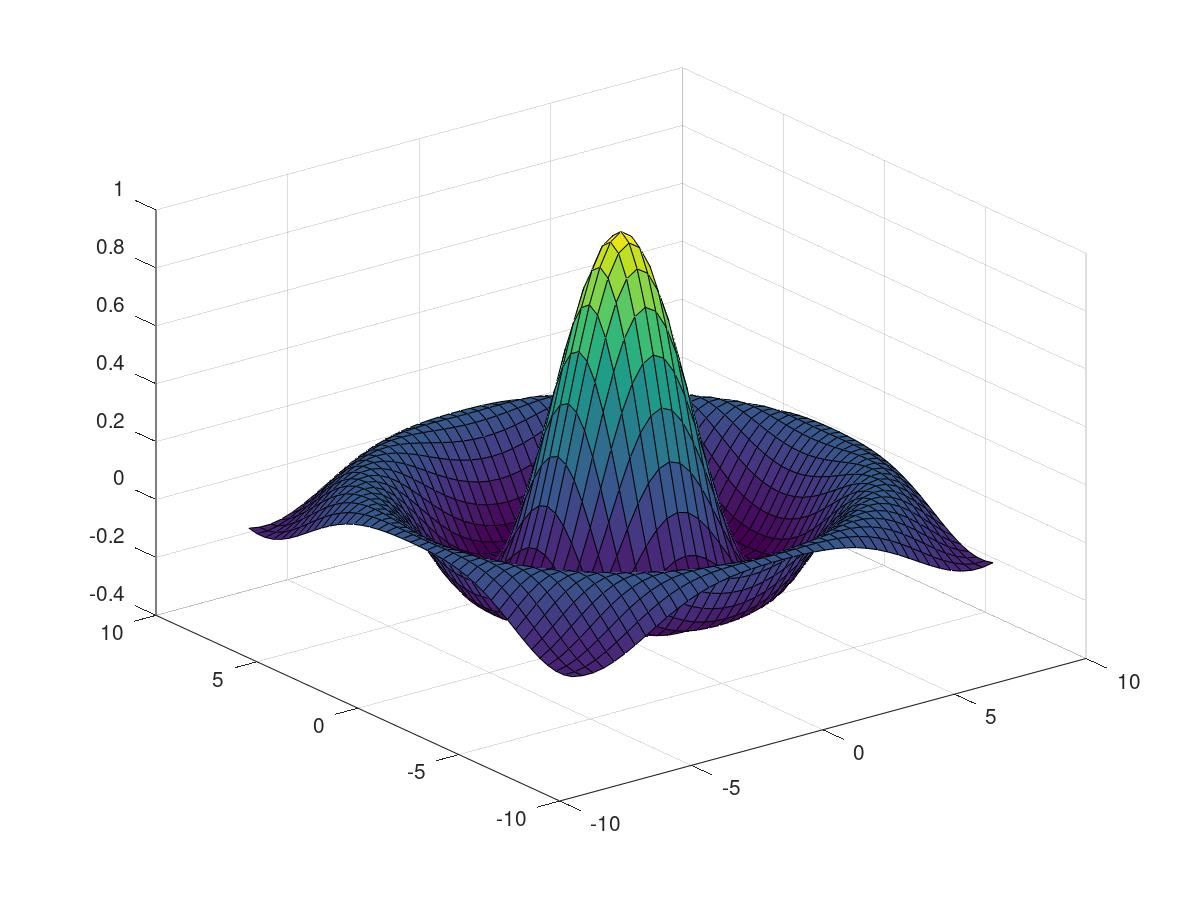
\includegraphics[width=\textwidth]{pub_example-1.jpg}
\end{figure}


\phantomsection
\addcontentsline{toc}{section}{matlab comment style ('\%') is supported as well \%}
\subsection*{matlab comment style ('\%') is supported as well \%}


\begin{itemize}
\item Bulleted list item 1
\item Bulleted list item 2
\end{itemize}
\begin{lstlisting}
%
         % # Numbered list item 1
         % # Numbered list item 2
\end{lstlisting}


\end{document}
